% Use class option [extendedabs] to prepare the 1-page extended abstract.
\documentclass[extendedabs]{bmvc2k}
\usepackage[colorlinks = true,
            linkcolor = blue,
            urlcolor  = blue,
            citecolor = blue,
            anchorcolor = blue]{hyperref}

% Document starts here
\begin{document}

\title{Learning From Massive Noisy Labeled Data for Image Classification}
\addauthor{
Tong Xiao$^1$, 
Tian Xia$^2$,
Yi Yang$^2$,
Chang Huang$^2$,
and Xiaogang Wang$^1$
}{}{1}
\addinstitution{
$^1$The Chinese University of Hong Kong.
$^2$Baidu Research.
}

\maketitle
\let\thefootnote\relax\footnote{This is an extended abstract. The full paper is available at the \href{http://www.cv-foundation.org/openaccess/CVPR2015.py}{Computer Vision Foundation webpage}. }
\vspace{-0.2in}

\noindent
Deep learning from large-scale supervised training dataset has shown very impressive improvement on image classification challenge~\cite{krizhevsky2012imagenet}. However, it requires reliable annotations from millions of images which are often expensive and time-consuming to obtain~\cite{deng2009imagenet}, preventing deep models from being quickly trained on new image recognition problems. Thus it is necessary to develop new efficient labeling and training frameworks for deep learning.

One possible solution is to automatically collect annotations from the Internet web images (\emph{i.e.} extracting tags from the surrounding texts) and directly use them as ground truth to train deep models. Unfortunately, these labels are extremely unreliable due to various types of noise (\emph{e.g.} labeling mistakes from annotators or computing errors from extraction algorithms). Many works have shown that noisy labels could adversely impact the classification accuracy of the induced classifiers~\cite{nettleton2010study}. Various label noise-robust algorithms~\cite{manwani2013noise} and data cleansing algorithms~\cite{brodley2011identifying} are developed but experiments show that performances are still affected by label noise~\cite{bartlett2006convexity}.

Although annotating all the data is costly, it is often easy to obtain a small amount of clean labels. Semi-supervised learning methods~\cite{lee2013pseudo} can be employed by simply discarding all the noisy labels. Researchers have also studied the transferability of Convolutional Neural Networks (CNNs) by finetuning an ImageNet pretrained model on smaller datasets of specific tasks~\cite{oquab2014learning}. However, these methods cannot fully utilize the massive noisy labeled data, which may lead to suboptimal results.

Our goal is to build an end-to-end deep learning system that is capable of training with both limited clean labels and massive noisy labels more effectively. Figure~\ref{fig:overview} shows the framework of our approach. We collect $1,000,000$ clothing images from online shopping websites. Each image is automatically assigned with a noisy label according to the keywords in its surrounding text. We manually refine $72,409$ image labels, which constitute a clean sub-dataset. All the data are then used to train CNNs, while the major challenge is to identify and correct wrong labels during the training process.

To cope with this challenge, we extend CNNs with a novel probabilistic model, which infers the true labels and uses them to supervise the training of the network. Our work is inspired by~\cite{sukhbaatar2014learning}, which modified a CNN by inserting a linear layer on top of the softmax layer to map clean labels to noisy labels. However,~\cite{sukhbaatar2014learning} assumed noisy labels are conditionally independent with input images given clean labels. By examining the collected dataset, we find that this assumption is too strong to fit real-world data well. For example, in Figure~\ref{fig:noise_cluster}, all the images should belong to ``Hoodie''. The top five are correct while the bottom five are either mislabeled as ``Windbreaker'' or ``Jacket''. Since different sellers have their own bias on different categories, they may provide wrong keywords for similar clothes. We can capture these visual patterns to estimate how likely an image is mislabeled. Based on these observations, we further introduce two types of label noise:
\begin{itemize}
\item \textbf{Confusing noise} makes the noisy label reasonably wrong. It usually occurs when the image content is confusing (\emph{e.g}, the samples with ``?'' in Figure~\ref{fig:overview}).
\item \textbf{Pure random noise} makes the noisy label totally wrong. It is often caused by either the mismatch between an image and its surrounding text, or the false conversion from the text to label (\emph{e.g.}, the samples with ``$\times$'' in Figure~\ref{fig:overview}).
\end{itemize}

Our proposed probabilistic model builds the relations among images, noisy labels, ground truth labels, and noise types, where the latter two are treated as latent variables. We use the Expectation-Maximization (EM) algorithm to solve the problem and integrate it into the deep learning framework. Experiments on the collected dataset show that our model can better detect and correct the wrong labels, which benefits the training of underlying CNNs.

\begin{figure}[t]
\begin{center}
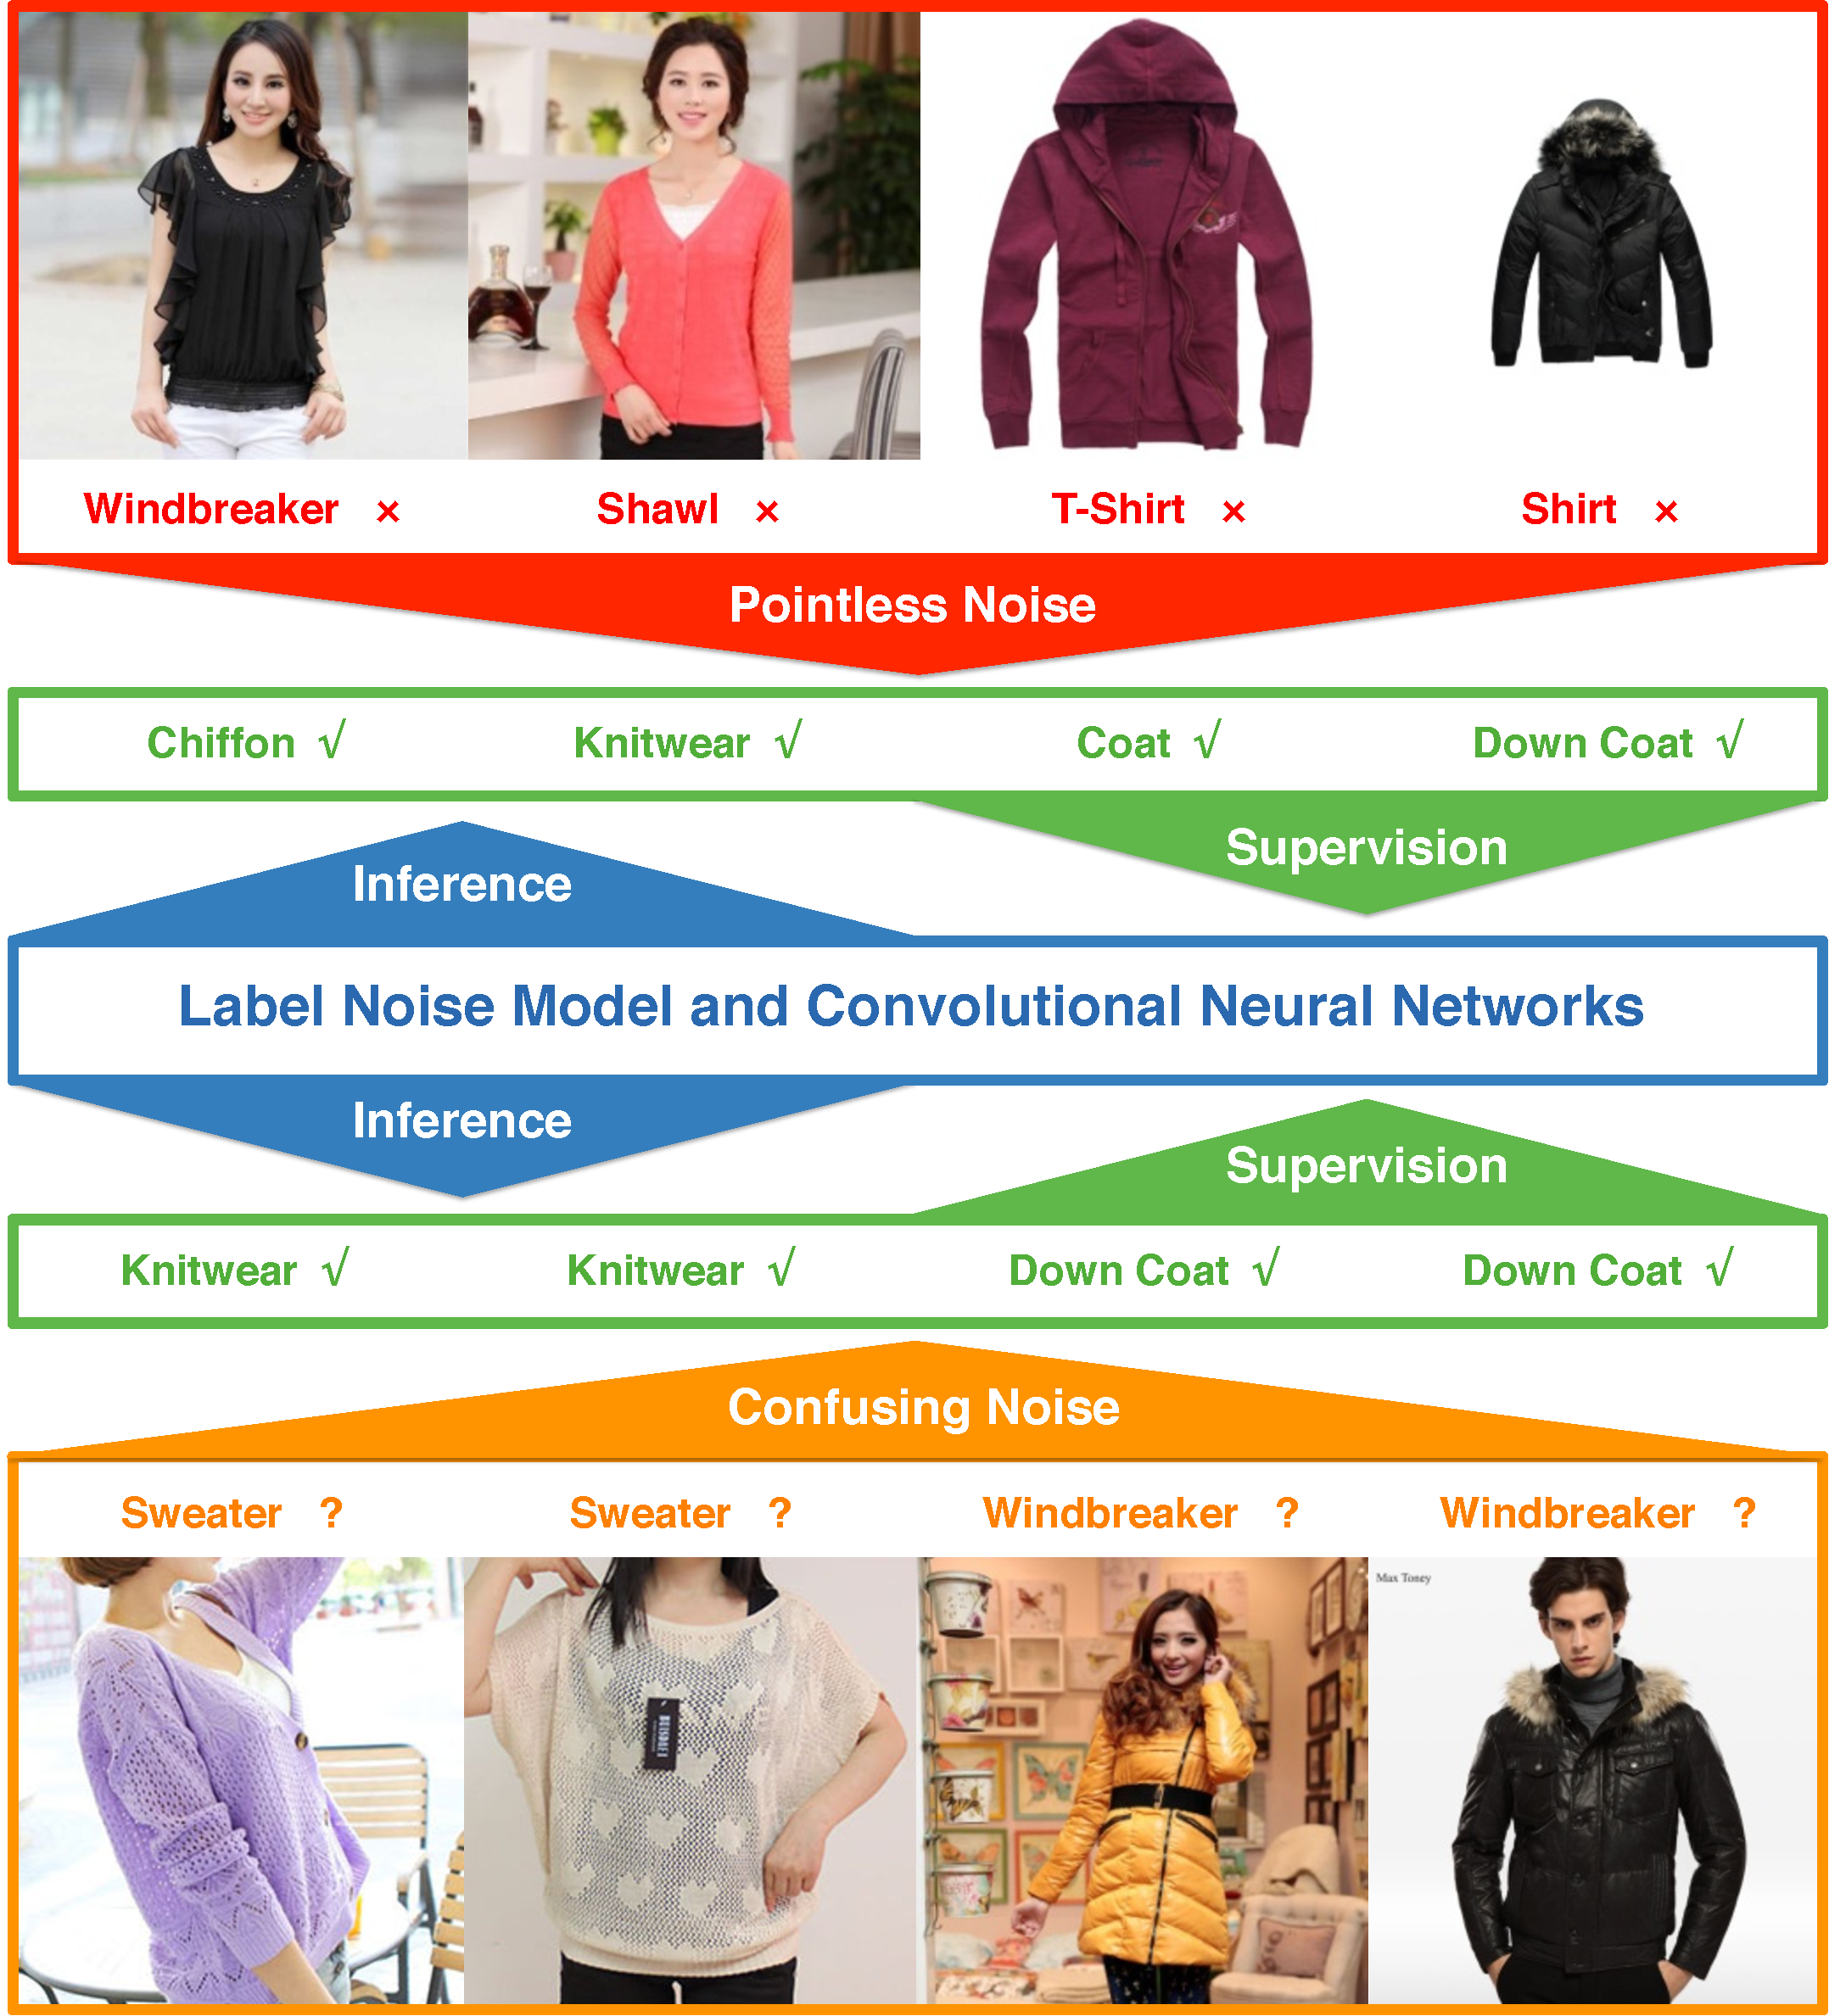
\includegraphics[width=0.8\linewidth]{figure/overview.pdf}
\end{center}
\caption{Overview of our approach. Labels of web images often suffer from different types of noise. A label noise model is proposed to detect and correct the wrong labels. The corrected labels are used to train underlying CNNs.}
\label{fig:overview}
\end{figure}

\begin{figure}[t]
\begin{center}
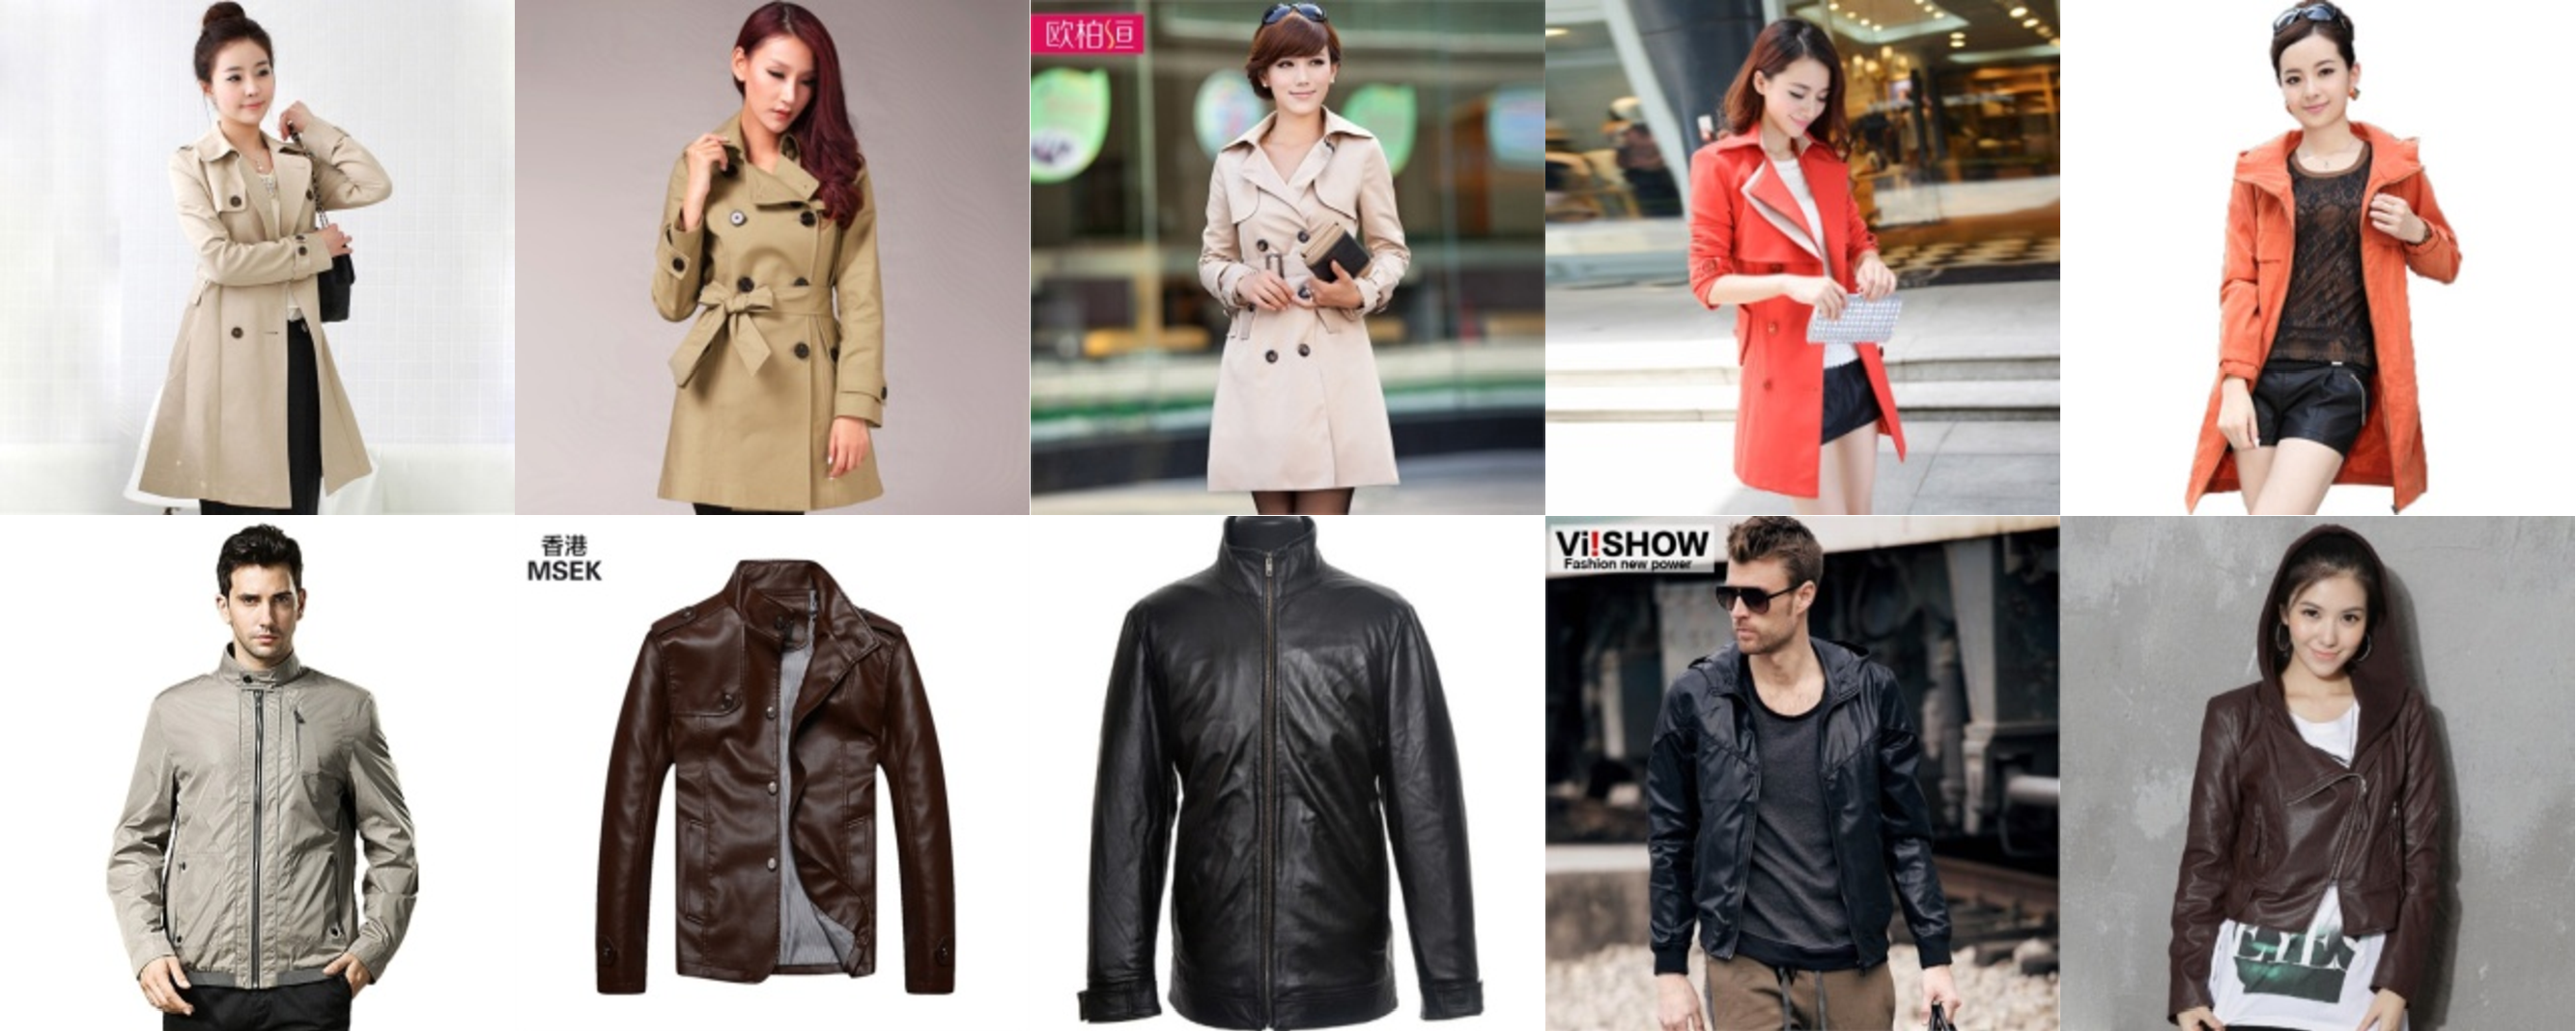
\includegraphics[width=0.8\linewidth]{figure/noise_cluster.pdf}
\end{center}
\caption{Mislabeled images often share similar visual patterns.}
\label{fig:noise_cluster}
\end{figure}

\bibliography{extbib}

\end{document}
